\chapter{Cassandra}
\label{chap:cassandra}
Cassandra ist die Quelle aller Daten von Twitter, die wir brauchen. Dazu werden die Daten direkt von der Twitter API über Kafka in Cassandra geladen und auf ein vorher für unsere Bedürfnisse zugeschnittenes Datenschema gemappt.

\section{Datenverwaltung}
Wir habe uns entschieden das Twitter Datenschema zu übernehmen. Da allerdings die Twitter Dokumentation nicht genau genug ist und nicht alle Attribute aller Datentypen übersichtlich darstellt, haben wir eine Applikation geschrieben, die sich Tweets vom Twitter Stream holt und daraus das Datenschema im Json Format zusammen baut. Nach dem wir die Applikation lange genug laufen lassen haben, hat sich an dem Datenschema nichts mehr geändert und wir konnten die Datentypen extrahieren.\\

\subsection{Datenschema}
Nach einer eingehenden Untersuchung aller möglichen Use Cases sind wir zum Schluss gekommen, dass uns fünf Tabelle alle Funktionen bieten die wir brauchen. Wir haben dabei zwei Tabellen für die User user\_by\_id und user\_by\_screen\_name entworfen wie man in Abbildung \ref{fig:schema}.
\begin{figure}
	\centering
	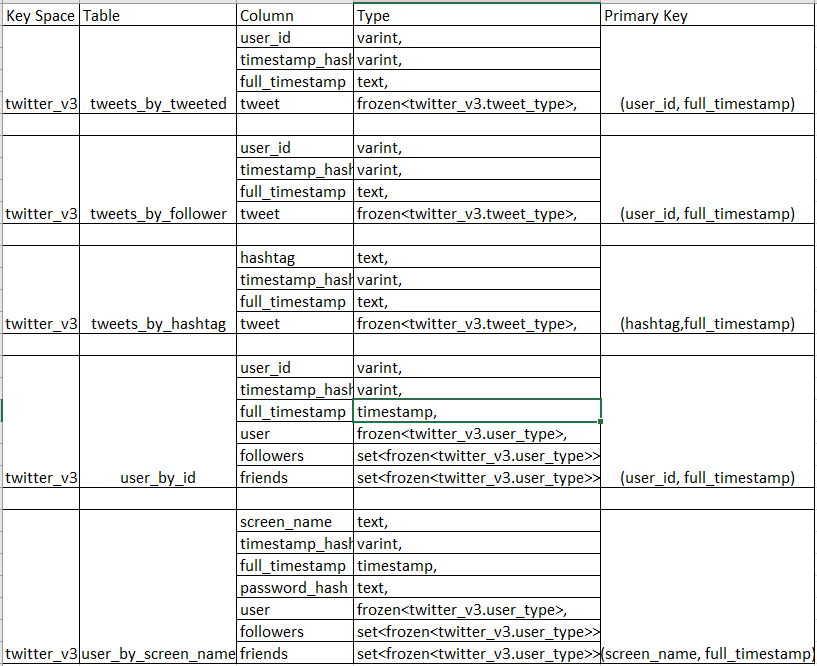
\includegraphics[scale=0.5, draft]{pics/schema.png}
	\caption{Cassandra Schema}
	\label{fig:schema}
\end{figure}
Da man bei Cassandra nur über den Primary Key (PK) auf Zeilen zugreifen und Bereichsabfragen über CQL machen kann, gilt es hier den PK so zu wählen, dass alle unsere Funktionen abgedeckt sind. Deshalb haben wir bei neben der User-Id für user\_by\_id und dem Screen-Name der Users für user\_by\_screen\_name auch den Timestamp mit aufgenommen. Da Cassandra leider keine vollständige Konsistenz bietet, müssen wir uns selber darum kümmern. Durch den Timestamp können wir verschiedene Versionen eines Objektes auseinander halten und die neuste bestimmen. Somit können wir zumindest einen gewissen Grad an Konsistenz bieten. Die weiteren Attribute der beiden Tabellen lassen sich einfach erklären. Die Follower und Friends eines Users sind wichtig, um die Timeline zu erstellen. Den password\_hash in user\_by\_screen\_name brauchen wir für den Login.\\
Die anderen drei Tabellen sind dafür da, die Tweets zu speichern und alle Tweet betreffenden Anfragen zu beantworten. Auch hier haben wir wieder den Timestamp bei allen Tabellen mit in den PK aufgenommen um Teilkonsistenz zu gewährleisten. tweets\_by\_tweeted speichert alle Tweets nach der User-Id des Users ab, der den Tweet abgesetzt hat. tweets\_by\_follower hingegen speichert einmal alle Tweets nach User-Id eines jeden Followers ab. Das Konzept hier ist es, durch die mehrfache Speicherung eines Tweets die Zeit bei der Abfrage nach allen Tweets, die ein User auf seiner Timeline sehen kann, zu verkürzen. Da man einmal abgesetzte Tweets auch nicht mehr ändern kann haben wir auch kein Problem damit jedes Objekt für Änderungen wieder heraussuchen zu müssen. tweets\_by\_hashtag speichert dann die Tweets danach ab, welche Hashtags in ihnen verwendet werden. Somit können auch Abfragen über Tweets eines Hashtags effizient beantwortet werden.

\section{Cassandrareader}
Die zentrale Applikation in der alle Funktionen und Schnittstellen umgesetzt werden ist der cassandrareader. Es ist eine modular aufgebaute in Java geschriebene Anwendung. Als Framework zur Unterstützung von verschiedenen Funktionen haben wir uns für SpringBoot entschieden. SpringBoot hat den Vorteil, dass es eine native API für Kafka besitzt, die es uns sehr leicht ermöglicht Publisher und Subscriber für Kafka-Topics zu schreiben. So ist die Verbindung mit Kafka sehr einfach konfigurierbar und kann innerhalb von kurzer Zeit verwendet werden. Für die Verbindung von Java zu Cassandra haben wir der DataStax Treiber genutzt \cite{DataStax}. Er biete eine generische Schnittstelle über die man mit Cassandra über CQL kommunizieren kann. Da er gut dokumentiert ist und es sehr viele Beispiele für verschiedene Anwendungen im Internet gibt, verlief die Einarbeitung in die Nutzung des DataStax Treibers sehr schnell.
\begin{figure}[htbp]
	\centering
	\includegraphics[scale=0.5, draft]{pics/cassandrareader_stack.png}
	\caption{Technologie Stack des cassandrareaders}
	\label{fig:techStackCass}
\end{figure}
Alle hier und im folgenden genutzten Bibliotheken werden über Maven eingebunden und der Applikation so zur Verfügung gestellt. Somit ist sichergestellt, dass immer die richtige Version geladen wird und keine Kompatibilitätsprobleme entstehen.

\subsection{Architektur}
Der Aufbau des Cassandrareaders ist sehr einfach gehalten wie man in Abbildung \ref{fig:archCass} sehen. Die Verbindung zu Cassandra wird vom Singleton CassandraConnector gemanaged. Diese Klasse stellt die Verbindung zu Cassandra her und bietet verschiedene Methoden an, Abfragen an Cassandra über CQL abzusetzen. Die eigentlich Funktion und Implementierung der Use Cases geschieht aber in den Kafka Subscribern. Dazu gibt es eine abstrakte Klasse AbstractKafkaSubscriber, die sozusagen die Infrastruktur bereitstellt. Diese besteht aus dem CassandraConnector, eine Gson-Instanz und mehreren Methoden, die die Optimierungen der Methoden aus dem Cassandra Connector darstellen, wie z.B. Batch-Queries und asynchrone Queries. Die Gson-Instanz kommt von der Google Gson Bibliothek, die für die JSON Konvertierung von Java Klasse zuständig ist. Sie wird in den abgeleiteten Klassen so benutzt, dass Kafka-Anfragen direkt in POJO Objekte gemappt werden, aus denen man dann alle relevanten Informationen bekommt. In den abgeleiteten Klassen wird dann auch die eigentliche Funktion eines Use Cases implementiert.
\begin{figure}[htbp]
	\centering
	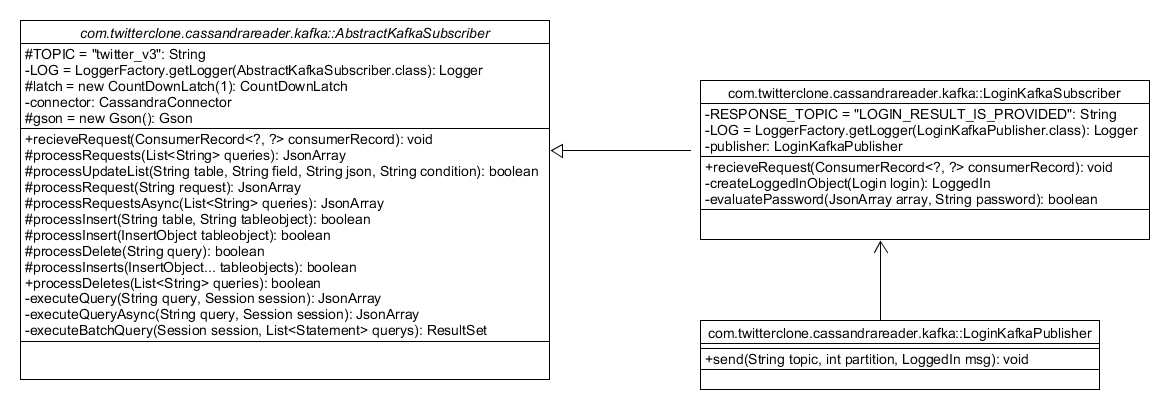
\includegraphics[scale=0.25, draft]{pics/cassandrareader_architecture.png}
	\caption{Technologie Stack des cassandrareaders}
	\label{fig:archCass}
\end{figure}
Alle möglichen Anfragen und Antworten über Kafka sind als Java Klassen modelliert und können über Getter-Methoden abgefragt werden. Jeder der abgeleiteten Subscriber besitzt einen Publisher, über den die Antwort, durch Gson konvertiert, wieder versendet werden kann. Die Konfigurationsparameter sind in der application.properties abgelegt und werden in den einzelnen Klassen angesprochen.


\section{Use Cases}
\label{sec:usecase}
Bei der Identifizierung der Use Cases die für Cassandra relevant sind haben wir uns für die Funktionen entschieden, die für einen Twitter-Client nach MVP-Prinzip (Minimal Viable Product) notwendig sind. Dabei haben wir vor allem die dazu gehören folgende Funktionen:
\begin{itemize}
	\item Registrierung von User
	\item Anmelden von Usern
	\item Abrufen der Timeline:
		\begin{itemize}
			\item Abfragen von Tweets
			\item Abfragen von Usern
		\end{itemize}
	\item Absenden/Speichern von Tweets
\end{itemize}
Diese Schnittstellen machen es möglich die Grundfunktionen, also das Erstellen eines Users, das Anmelden, das Senden von Tweets und das Lesen von Tweets über die Timeline von außen über vordefinierte Kafka Nachrichten anzusprechen.
Als weitere Schnittstellen für erweiterte Funktionen haben wir eine API für Volltextsuche über Elasticsearch gebaut, die die normale Volltextsuche aber auch Autocompletion unterstützt.\\ \TODO{vielleicht deletion hinzufügen}




\subsection{Registrierung von Usern}

\subsection{Anmelden von Usern}

\subsection{Abfragen von Tweets}

\subsection{Abfragen von Usern}

\subsection{Abrufen der Timeline}

\subsection{Absenden/Speichern von Tweets}
